\documentclass{article}

\PassOptionsToPackage{numbers,compress}{natbib}
\usepackage[dblblindworkshop,final]{neurips_2026}
\workshoptitle{Machine Learning and the Physical Sciences}
\makeatletter
\renewcommand{\@noticestring}{9th Workshop on Machine Learning and the Physical Sciences (ML4PS 2026).}
\makeatother

\usepackage[utf8]{inputenc}
\usepackage[T1]{fontenc}
\usepackage{amsmath}
\usepackage{amsfonts}
\usepackage{hyperref}
\usepackage{url}
\usepackage{booktabs}
\usepackage{nicefrac}
\usepackage{microtype}
\usepackage{xcolor}
\usepackage{graphicx}
\usepackage{placeins}

\newcommand{\Msun}{M_\odot}
\newcommand{\Lt}{\tilde{\Lambda}}
\newcommand{\Mc}{\mathcal{M}}

\title{Amortized Multi-Messenger Neutron-Star Equation-of-State Inference via Heterogeneous Set Aggregation}

\author{%
  Soham Lohar\textsuperscript{1} \quad Raehan Baliga\textsuperscript{2} \quad Virat Varada\textsuperscript{5}\\
  \textbf{Aaditya Bilakanti\textsuperscript{3} \quad Ryan Bui\textsuperscript{4}}\\[4pt]
  \textsuperscript{1}\href{https://westview.beaverton.k12.or.us/}{Westview High School} \quad
  \textsuperscript{2}\href{https://www.lwsd.org/}{Lake Washington School District}\\
  \textsuperscript{3}\href{https://exeter.edu/}{Phillips Exeter Academy} \quad
  \textsuperscript{4}\href{https://uci.edu/}{University of California, Irvine} \quad
  \textsuperscript{5}Independent}

\begin{document}
\maketitle

\begin{abstract}
Combining a growing, heterogeneous catalog of neutron-star observations into one equation-of-state (EOS) posterior normally requires a new sampling run for every catalog. We amortize this step with a single network. Type-specific encoders embed gravitational-wave, NICER and radio-timing observations with their uncertainties, a Set Transformer aggregates catalogs of any size (1--50) and any messenger mix, and a flow-matching decoder returns the full posterior over a four-parameter spectral EOS in under a second. Validated against nested sampling run on the exact likelihood of the same simulator, the amortized posterior is statistically indistinguishable on real data: Jensen--Shannon divergence $\le0.0014$ bits, at the sampling-noise floor, and a joint two-sample test at chance (0.49). The real catalog gives $R_{1.4}=12.22^{+0.72}_{-0.76}$\,km and $M_{\rm TOV}=2.54^{+0.34}_{-0.33}\,\Msun$. The network is calibrated to within 1.3 points across 15,000 held-out catalogs, matches nested sampling on 24 synthetic catalogs, and can be made exact by importance reweighting at 86\% efficiency, which also yields the Bayesian evidence. It is $139\times$ faster per catalog ($774\times$ per effective sample) and analyzes all 127 sub-catalogs of the real data in 24\,s instead of ${\sim}4$\,h. Controlled ablations show the Set Transformer outperforming DeepSets and padded-MLP aggregators. An estimator-independent analysis reveals that current observables constrain only two of the four EOS coefficients.
\end{abstract}

\section{Introduction}

The equation of state (EOS) of matter above nuclear saturation density is a central open question in nuclear astrophysics. Neutron stars constrain it through complementary channels: GW tidal deformabilities from binary mergers \citep{abbott2017gw170817,abbott2020gw190425}, NICER mass--radius measurements from pulse-profile modeling \citep{miller2019psr,riley2019nicer,miller2021radius,riley2021nicer,choudhury2024j0437}, and pulsar masses from radio timing and optical spectroscopy \citep{demorest2010twosolar,fonseca2021refined,romani2022psr}. Combining these into one EOS posterior is usually done with likelihood-based sampling \citep{ashton2019bilby,speagle2020dynesty} or hierarchical inference \citep{golomb2022hierarchical,ray2023rapid}, which must be rerun whenever the catalog changes. Neural posterior estimation (NPE) \citep{cranmer2020frontier} has made single-event GW inference fast \citep{dax2021real,dax2025realtime} and has been applied to EOS inference from stellar observables \citep{carvalho2025neural}.

We treat the \emph{combination} step itself as a set-conditioned NPE problem. Our contributions are:
\begin{itemize}\setlength\itemsep{1pt}
\item To our knowledge, the first amortized EOS posterior that aggregates heterogeneous multi-messenger catalogs with a Set Transformer. One network takes 1--50 observations mixing GW, NICER and radio/optical masses, each with its own noise level, and serves any catalog size and messenger composition without retraining.
\item Validation against nested sampling with the simulator's mass-marginalized likelihood on a validated TOV grid. We derive the exact marginal likelihood of the simulator, test it against Monte Carlo, and compare to nested sampling on real and synthetic catalogs with sample-size-matched divergences and a joint two-sample test. An importance-sampling correction \citep{dax2023neural} targets the posterior defined by this gridded likelihood.
\item Controlled architecture and messenger ablations, calibration on 15,000 catalogs, and an estimator-independent identifiability analysis of the spectral EOS.
\item An explicit cost model: offline cost, break-even, and a workflow that amortization makes practical.
\end{itemize}

\section{Method}

\paragraph{EOS and forward model.} Below $3\,$MeV\,fm$^{-3}$ we use the SLy4 table \citep{douchin2001unified}. Above it, the adiabatic index follows the spectral form $\Gamma(x)=\exp(\gamma_0+\gamma_1x+\gamma_2x^2+\gamma_3x^3)$ \citep{lindblom2010spectral}, with $x=\ln(P/P_0)/\ln(P_{\max}/P_0)\in[0,1]$. At the first causal crossing we continue the EOS at $c_s=c$. If the spectral EOS remains causal up to $P_{\max}=1500\,$MeV\,fm$^{-3}$, we continue it at its terminal sound speed. We integrate the TOV and tidal (Love-number) equations \citep{hinderer2008tidal} at 30 central pressures. A deterministic step budget makes acceptance independent of machine load, and the maximum mass $M_{\rm TOV}$ is located by bracketing the peak of the mass sequence. Against a $4\times$ denser, $100\times$ tighter solve, the 95th-percentile radius error is 0.011\,km (4\% of the smallest training $\sigma_R$). The prior is uniform on $\gamma_0\in[0.2,2]$, $\gamma_1\in[-1.6,1.7]$, $\gamma_2\in[-0.6,0.6]$, $\gamma_3\in[-0.02,0.02]$, truncated to EOSs with $M_{\rm TOV}\ge1.5\,\Msun$ (63.5\% acceptance). This cut is deliberately below the heaviest observed pulsars, so that pulsar masses constrain $M_{\rm TOV}$ through the likelihood rather than the prior.

\paragraph{Simulator.} A catalog has $N\sim\mathcal{U}\{1,\dots,50\}$ observations, a Dirichlet-multinomial messenger mix ($\alpha=\mathbf{1}$, so messengers may be absent) and random order. GW events have component masses $m_{1,2}\sim\mathcal{U}(1.1,\min(M_{\rm TOV},2))$ and are observed as $(\Lt,\Mc)$ with Gaussian noise. NICER sources have $m\sim\mathcal{U}(1.2,\min(M_{\rm TOV},2.2))$ and are observed as $(M,R(m))$. Pulsars have $m\sim\mathcal{U}(1.4,\min(M_{\rm TOV},2.5))$ and are observed as $M$. Every noise scale is drawn log-uniformly and independently of $\theta$: $\sigma_{\Lt}\in[40,800]$, $\sigma_{\Mc}\in[5\!\times\!10^{-4},0.03]$, $\sigma_M^{\rm NICER}\in[0.02,0.2]$, $\sigma_R\in[0.3,1.6]$\,km, $\sigma_M^{\rm PSR}\in[0.01,0.25]$. The ranges cover the real data. We simulate 100,000 accepted EOSs (70/15/15 split) and redraw the catalog of each EOS every epoch.

\paragraph{Architecture.} Each messenger has a three-layer GELU MLP that embeds its observation and standardized $\log\sigma$ (GW and NICER: 4 inputs; pulsars: 2) into $\mathbb{R}^{256}$, plus a learned type embedding. A six-layer Set Transformer \citep{lee2019set} (8 heads) with attention pooling produces a permutation-invariant summary $s$, to which $\ln(1+N)$ is appended. Shuffling or padding a catalog changes the network output by $\le2\times10^{-6}$. A residual velocity network (4 blocks, width 512) is trained with conditional flow matching \citep{lipman2023flow,wildberger2023flow}, $\mathcal{L}=\mathbb{E}\,\|v_\phi(x_t,t,s)-(\theta-z)\|^2$ with $x_t=(1-t)z+t\theta$. Samples are drawn by 50-step RK4 integration, which shifts posterior medians by $<10^{-4}$ posterior standard deviations relative to 100 steps. Samples are kept only inside the prior box. Training uses AdamW (learning rate $3\times10^{-4}$, weight decay $10^{-4}$), batch size 256, cosine decay, and early stopping on a fixed-seed validation set (patience 40, at most 400 epochs). The headline model is a 3-seed ensemble ($7.7$M parameters each; best epochs 367, 396 and 115). Architecture hyperparameters were fixed before evaluation and not tuned on test data.

\paragraph{Exact reference likelihood.} The network and the reference must target the same posterior. We therefore write the simulator's marginal likelihood exactly. The GW term marginalizes $m_{1,2}$ by quadrature. NICER and pulsar terms marginalize the true mass over its uniform prior, which gives a closed form for pulsars. The prior includes the same truncation. Each term is tested against brute-force Monte Carlo of the simulator. Macroscopic curves come from a $20\times20\times10\times5$ TOV grid, interpolated and validated on held-out EOSs. We sample this likelihood with dynesty \citep{speagle2020dynesty} (500 live points, random-walk proposals, two seeds for the primary real catalog and one run with the duplicate J0740+6620 mass). We compare marginals with Jensen--Shannon (JS) divergence in bits, computed with KDE on matched sample sizes (the dynesty effective sample size). Each divergence is reported with its finite-sample floor (JS between independent draws from one method). We also report a classifier two-sample test (C2ST) \citep{lopezpaz2017revisiting} on the joint 4-D posterior. The same likelihood drives an importance-sampling correction: a defensive mixture of the flow (90\%) and the uniform box prior (10\%) serves as the proposal, with the flow density obtained by the continuous change of variables. This gives efficiency, effective sample size and evidence.

\paragraph{Real catalog.} For GW170817 and GW190425 we summarize $(\Lt,\Mc)$ from the public low-spin samples in the \href{https://dcc.ligo.org/LIGO-P1800370/public}{GWTC-1} and \href{https://dcc.ligo.org/LIGO-P2000026/public}{GW190425} releases, respectively. The NICER inputs are PSR~J0030+0451 \citep{riley2019nicer}, J0740+6620 \citep{riley2021nicer}, and J0437$-$4715 \citep{choudhury2024j0437}. Mass measurements come from optical spectroscopy of J0952$-$0607 \citep{romani2022psr} and radio timing of J1614$-$2230 ($1.908\pm0.016\,\Msun$, Table~8 of Arzoumanian et al.~\citep{arzoumanian2018timing}). The primary catalog uses J0740+6620's timing information once, through the NICER mass prior. A sensitivity run adds the radio mass separately \citep{fonseca2021refined}. All seven observations pass our marginal training-range check.

\section{Results}

\begin{figure}[t]
\centering
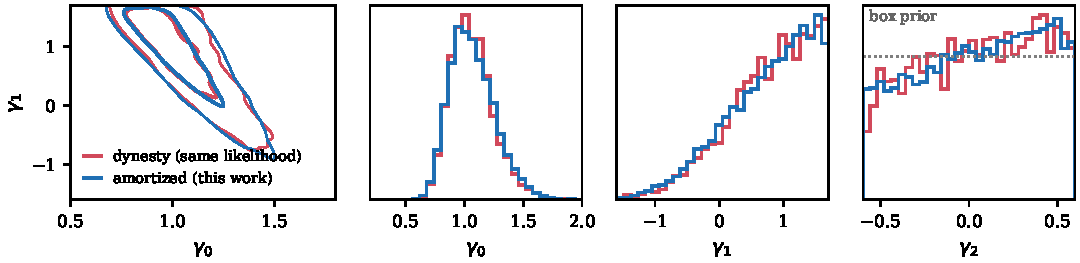
\includegraphics[width=\linewidth]{figures/real_posterior.pdf}\\[2pt]
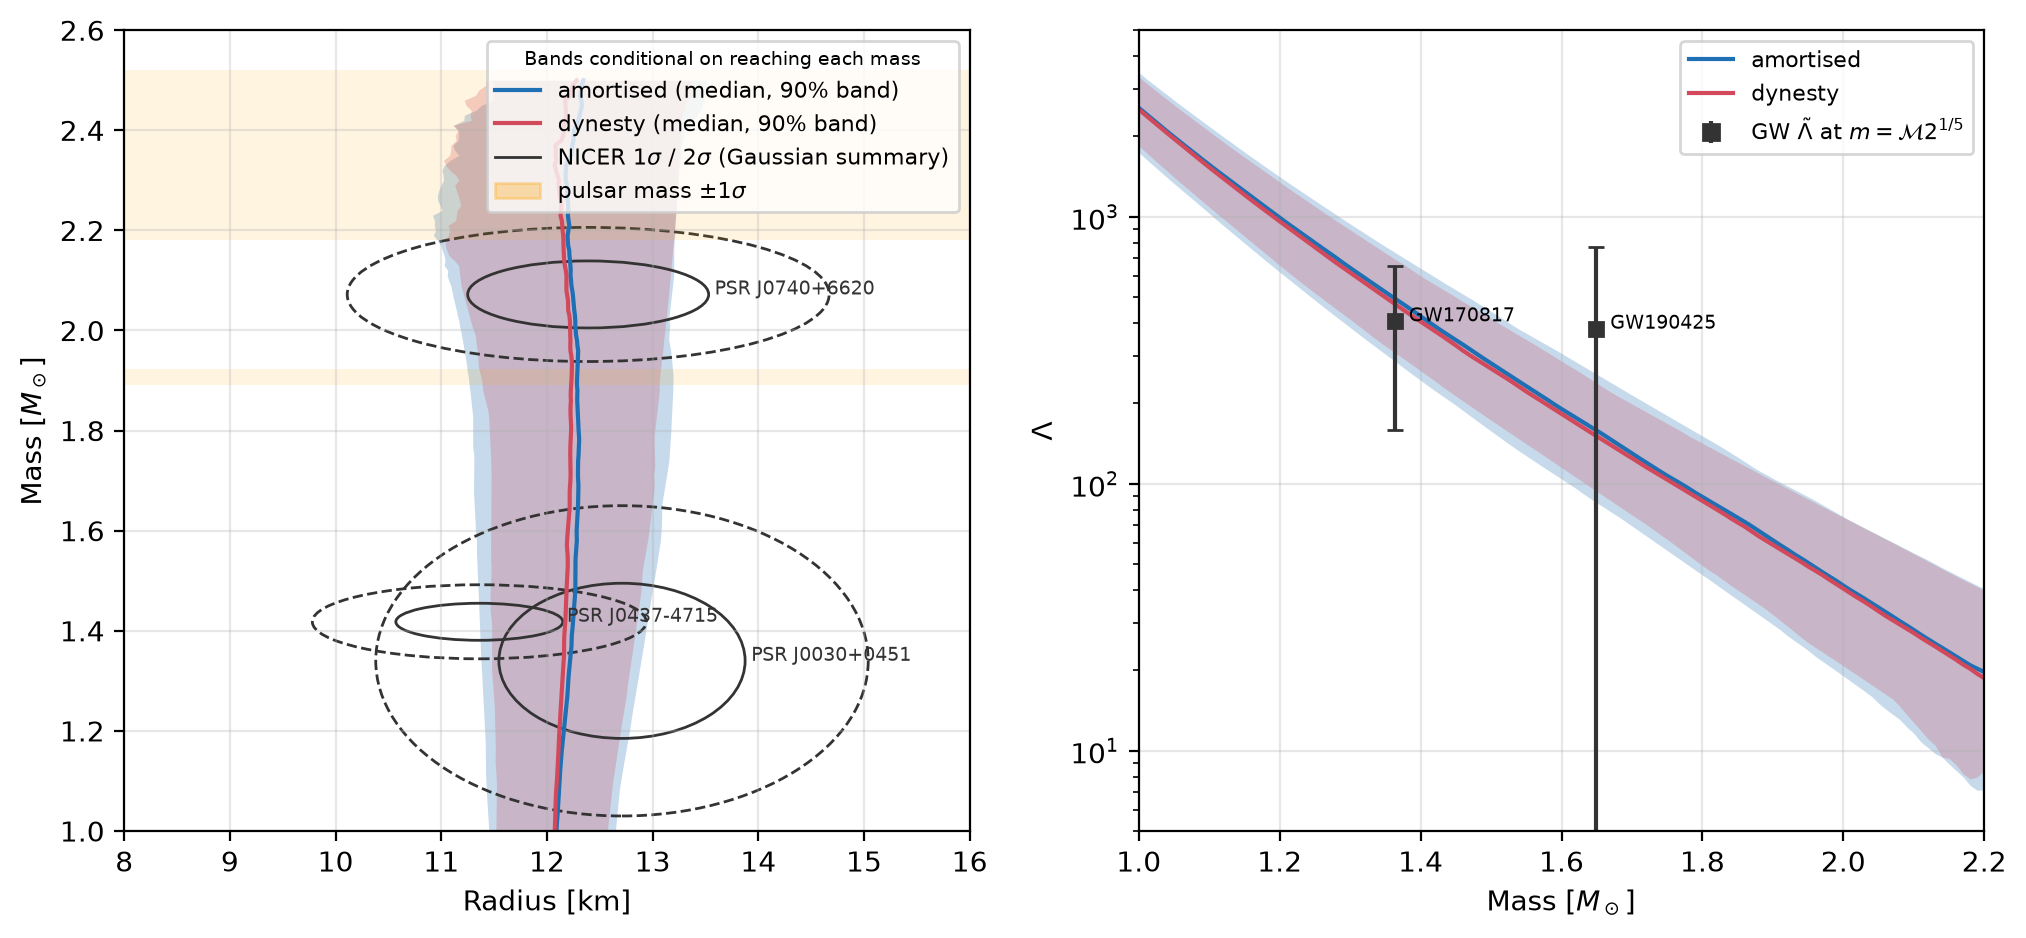
\includegraphics[width=0.92\linewidth]{figures/fig1_mr_mlambda.png}
\caption{Real seven-observation catalog. \textbf{Top:} amortized posterior (blue, 0.84\,s) vs.\ dynesty with the identical likelihood (red, 117\,s). The $\gamma_0$--$\gamma_1$ panel shows 50\%/90\% contours. $\gamma_2$ is close to the prior, and $\gamma_3$ (not shown) matches the prior. \textbf{Bottom:} implied mass--radius and mass--$\Lambda$ bands (median, 90\%) with the NICER and pulsar inputs.}
\label{fig:real}
\end{figure}

\paragraph{Real data: posterior fidelity.} The amortized and nested-sampling posteriors agree to the precision of the comparison (Fig.~\ref{fig:real}, Table~\ref{tab:real}). Marginal JS divergences are 0.0008--0.0014 bits, no larger than the network's own finite-sample floor. C2ST accuracy on the joint posterior is 0.490 (dynesty against itself: 0.497). Every posterior mean agrees within $0.033\,\sigma$, and pairwise correlations agree within 0.035, including the strong $\gamma_0$--$\gamma_1$ anticorrelation. The derived observables agree to $\le0.03$\,km and $\le0.01\,\Msun$. Our $R_{1.4}=12.22\,[11.46,12.94]$\,km overlaps the $12.45\pm0.65$\,km range spanning the 68\% intervals of three EOS frameworks in Miller et al.~\citep{miller2021radius}. Abbott et al.~\citep{abbott2018radii} obtained compatible radii from GW170817. The upper tail of $M_{\rm TOV}=2.54\,[2.21,2.88]\,\Msun$ depends on the causal continuation: only 5.2\% of the importance-weighted posterior reaches its mass peak within the causal spectral domain. Conditioning on this subset gives $M_{\rm TOV}=2.27\,[2.07,2.52]\,\Msun$ and shifts median $R_{1.4}$ from 12.18 to 12.67\,km. Importance reweighting for the grid-based likelihood retains 86\% efficiency (ESS 17,242 of 20,000). For the prior normalized over accepted EOSs, $\ln Z=-18.618\pm0.004$ from reweighting and $-18.562\pm0.065$ from dynesty.

\begin{table}[t]
\caption{Real catalog, amortized vs.\ dynesty (same likelihood). JS divergence in bits on matched samples ($n{=}1{,}802$, 200 subsample repeats). Floor: JS between independent amortized sample sets. Derived quantities: median and 90\% interval.}
\label{tab:real}
\centering\small\setlength\tabcolsep{5pt}
\begin{tabular}{lcccc}
\toprule
 & $\gamma_0$ & $\gamma_1$ & $\gamma_2$ & $\gamma_3$ \\
\midrule
JS, amortized vs.\ dynesty [bits] & 0.0014 & 0.0011 & 0.0008 & 0.0008 \\
JS floor [bits] & 0.0017 & 0.0012 & 0.0008 & 0.0008 \\
$(\mu_{\rm amort}-\mu_{\rm dyn})/\sigma_{\rm dyn}$ & $+0.02$ & $-0.03$ & $-0.03$ & $-0.01$ \\
$\sigma_{\rm amort}/\sigma_{\rm dyn}$ & 1.04 & 1.03 & 1.02 & 0.99 \\
\midrule
 & \multicolumn{2}{c}{amortized} & \multicolumn{2}{c}{dynesty} \\
\midrule
$R_{1.4}$ [km] & \multicolumn{2}{c}{12.22 [11.46, 12.94]} & \multicolumn{2}{c}{12.19 [11.48, 12.95]} \\
$\Lambda_{1.4}$ & \multicolumn{2}{c}{418 [261, 640]} & \multicolumn{2}{c}{413 [265, 638]} \\
$M_{\rm TOV}$ [$\Msun$] & \multicolumn{2}{c}{2.54 [2.21, 2.88]} & \multicolumn{2}{c}{2.55 [2.24, 2.89]} \\
C2ST accuracy, joint 4-D & \multicolumn{2}{c}{0.490} & \multicolumn{2}{c}{floor 0.497} \\
\bottomrule
\end{tabular}
\end{table}

\paragraph{Synthetic catalogs: fidelity and calibration.} The single real catalog is not the only test. We ran dynesty on 24 synthetic catalogs stratified by size ($N\in[1,20]$). Median JS divergences were 0.0012--0.0027 bits (within $2\times$ the floor), median C2ST 0.519 (floor 0.504), and posterior widths were 97--98\% of the reference. The highest C2ST accuracy was 0.648 and fell to 0.479 after importance reweighting on that catalog. Importance reweighting on these catalogs gave a median efficiency of 82\% and median $|\Delta\ln Z|=0.05$. On 15,000 held-out catalogs, rank histograms are flat. Coverage at the 50/68/90/95\% levels is within 1.3 percentage points of nominal for every parameter, and within 0.30 points on average for the identifiable $\gamma_0,\gamma_1$ (Fig.~\ref{fig:calib}a). A slight tail under-coverage remains (93.8--94.8\% at 95\%), and the joint TARP test \citep{lemos2023sampling} deviates by at most 0.029. In observable space (100 catalogs, TOV solved for each posterior draw), $M_{\rm TOV}$, $R_{1.4}$ and $\Lambda_{1.4}$ have 68\% coverage of 66/71/68\%, with errors $3.6\times$, $5.7\times$ and $5.3\times$ smaller than the prior's. Information increases monotonically with catalog size up to $N=50$, now inside the training range (Fig.~\ref{fig:calib}b). Inference time does not depend on $N$: 0.39\,s for 1,000 draws at $N=1$ and at $N=50$.

\begin{figure}[t]
\centering
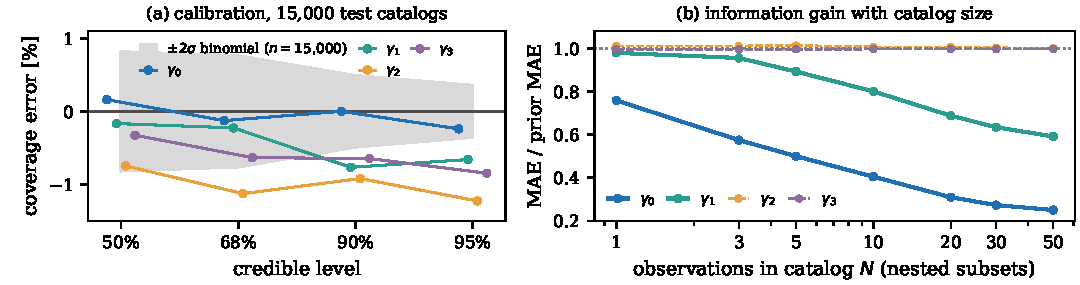
\includegraphics[width=\linewidth]{figures/calibration_scaling.pdf}
\caption{(a) Empirical minus nominal coverage of central credible intervals on 15,000 held-out catalogs. (b) Posterior-median error relative to the prior, for nested subsets of the same catalogs: adding observations to a fixed EOS steadily sharpens $\gamma_0$ and $\gamma_1$, while $\gamma_2$ and $\gamma_3$ stay at the prior.}
\label{fig:calib}
\end{figure}

\paragraph{Ablations.} All architecture arms use the same flow-matching decoder, data and budget (150 epochs), with three seeds each (Table~\ref{tab:ablate}). Replacing the set encoder with a padded MLP over a fixed-size vector increases error by 12\% ($\gamma_0$) and 9\% ($\gamma_1$) and worsens calibration. The Set Transformer is best on every metric. Its margin over DeepSets \citep{zaheer2017deep} in validation loss (0.0046) is ${\sim}20\times$ the seed-to-seed spread, so attention-based aggregation gives a consistent gain over sum pooling. All arms received the same 150-epoch budget. For messengers, we use fixed catalogs of six observations. GW-only and NICER-only catalogs are about equally informative (prior-relative error on $\gamma_0$: 0.37 and 0.38), while pulsar masses alone carry little information (0.88). Models retrained on a single messenger match the main model to within 0.005, so one network serves every messenger mix without loss.

\begin{table}[t]
\caption{\textbf{Left:} architecture ablation (mean of 3 seeds; error relative to the prior MAE on 4,000 test catalogs; mean $|$coverage error$|$). \textbf{Right:} identifiability: near-zero-noise flow model; $R^2$ of a gradient-boosting regressor \citep{friedman2001greedy} on noise-free $M$--$R$--$\Lambda$ curves; Fisher posterior/prior width at current precision; change in $R_{1.4}$ across the full prior range of each parameter.}
\label{tab:ablate}
\centering\footnotesize\setlength\tabcolsep{3.5pt}
\begin{tabular}{lcccc}
\toprule
encoder (params) & val.\ loss & $\gamma_0$ & $\gamma_1$ & cov.\ err. \\
\midrule
Set Transformer (7.7M) & \textbf{1.0923} & \textbf{0.324} & \textbf{0.720} & \textbf{0.91\%} \\
DeepSets (2.7M) & 1.0969 & 0.327 & 0.726 & 0.94\% \\
padded MLP (3.6M) & 1.1311 & 0.363 & 0.787 & 1.05\% \\
\bottomrule
\end{tabular}\hfill
\begin{tabular}{lcccc}
\toprule
 & $\gamma_0$ & $\gamma_1$ & $\gamma_2$ & $\gamma_3$ \\
\midrule
zero-noise err.\ ratio & 0.03 & 0.13 & 0.66 & 1.00 \\
regressor $R^2$ & 1.00 & 0.97 & 0.27 & 0.00 \\
Fisher width ratio & 0.37 & 0.76 & 0.99 & 1.00 \\
$\Delta R_{1.4}$ [km] & 3.24 & 0.99 & 0.23 & 0.002 \\
\bottomrule
\end{tabular}
\end{table}

\paragraph{Identifiability.} With realistic noise, $\gamma_2$ and $\gamma_3$ are not learned: test error equals the prior's (ratios 0.98 and 1.00) and posterior contraction is below 0.05. Three independent checks show that this is a property of the forward map, not of the estimator (Table~\ref{tab:ablate}, right). A flow trained at near-zero noise recovers $\gamma_0$ and $\gamma_1$ almost perfectly, $\gamma_2$ only partially, and $\gamma_3$ not at all. A model-free regressor on noise-free curves reaches $R^2=0.27$ for $\gamma_2$ and $0$ for $\gamma_3$. A Fisher analysis finds one well-constrained direction at current precision. Physically, sweeping $\gamma_3$ across its whole prior range moves $R_{1.4}$ by 2\,m. The model is therefore effectively two-parameter for current data, within the adopted prior. Lindblom and Indik~\citep{lindblom2014spectral} studied the accuracy of low-order spectral reconstructions using mock stellar data.

\paragraph{Speed and workflows.} The amortized posterior for the real catalog takes 0.84\,s, against 117\,s for dynesty: $139\times$ faster in wall clock and $774\times$ per effective sample. Importance correction takes 38\,s, a $3.06\times$ wall-clock speed-up over dynesty. The speed-up turns analyses that were impractical into routine ones. All 127 sub-catalogs of the real data take 24\,s, against 4.1\,h extrapolated from 127 runs at the full-catalog dynesty time, and give the influence of each observation directly: removing PSR~J0437$-$4715 shifts $R_{1.4}$ the most ($+0.29$\,km). The same applies to observation planning and large injection campaigns. The one-time cost is 14.4\,h of simulation on 16 CPU threads and 5.7\,h of training on one RTX~5070, recovered after ${\sim}570$ analyses.

\section{Limitations and conclusion}

\textbf{Robustness to misspecification.} When the true noise scales were $1.3\times$ the reported values, the largest mean absolute coverage error was 2.1 percentage points. Across 500 paired catalogs, the nominal 90\% interval for $\gamma_0$ covered the truth in 90.0\% of cases with the training crust (SLy4) and 57.2\% with a randomized polytropic crust. A crust-marginalized model is future work. We approximate the GW and NICER measurements with independent Gaussian summaries. Extending the encoders to posterior samples is one direction for future work. Robust inference and model checks for simulator mismatch offer complementary approaches \citep{ward2022robust,schmitt2024detecting}. As with any amortized method, changing the prior, noise model or simulator requires re-simulation and retraining.

\textbf{Conclusion.} A single set-conditioned flow-matching posterior reproduces nested sampling with the same likelihood on real and synthetic multi-messenger catalogs, is calibrated across catalog sizes and messenger mixes, and can be reweighted to target the grid-based reference posterior. Validated this way, amortization turns repeated EOS analyses from hours into seconds, and it shows directly which EOS parameters current data can constrain.

\begin{ack}
% PLACEHOLDER -- edit to reflect your actual funding and support.
This revision substantially changes the submitted version: the simulator, likelihood, reference sampler and all experiments were rebuilt and rerun after the reviews, and the numbers in the submitted version are superseded. The authors take responsibility for all content.
\end{ack}

\begin{thebibliography}{99}\small\setlength\itemsep{0pt}

\bibitem{abbott2017gw170817} B.~P.~Abbott et al.\ (LVC). GW170817: Observation of gravitational waves from a binary neutron star inspiral. \emph{Phys.\ Rev.\ Lett.}, 119:161101, 2017.

\bibitem{abbott2018radii} B.~P.~Abbott et al.\ (LVC). GW170817: Measurements of neutron star radii and equation of state. \emph{Phys.\ Rev.\ Lett.}, 121:161101, 2018.

\bibitem{abbott2020gw190425} B.~P.~Abbott et al.\ (LVC). GW190425: Observation of a compact binary coalescence with total mass $\sim3.4\,\Msun$. \emph{Astrophys.\ J.\ Lett.}, 892:L3, 2020.

\bibitem{arzoumanian2018timing} Z.~Arzoumanian et al. \href{https://doi.org/10.3847/1538-4365/aab5b0}{The NANOGrav 11-year data set: High-precision timing of 45 millisecond pulsars}. \emph{Astrophys.\ J.\ Suppl.}, 235:37, 2018.

\bibitem{ashton2019bilby} G.~Ashton et al. BILBY: A user-friendly Bayesian inference library for gravitational-wave astronomy. \emph{Astrophys.\ J.\ Suppl.}, 241:27, 2019.

\bibitem{carvalho2025neural} V.~Carvalho, M.~Ferreira, M.~Bejger, and C.~Provid\^encia. Neural posterior estimation of neutron star equations of state. \emph{Phys.\ Rev.\ D}, 112:083044, 2025.

\bibitem{choudhury2024j0437} D.~Choudhury et al. A NICER view of the nearest and brightest millisecond pulsar: PSR J0437$-$4715. \emph{Astrophys.\ J.\ Lett.}, 971:L20, 2024.

\bibitem{cranmer2020frontier} K.~Cranmer, J.~Brehmer, and G.~Louppe. The frontier of simulation-based inference. \emph{PNAS}, 117:30055--30062, 2020.

\bibitem{dax2021real} M.~Dax et al. Real-time gravitational wave science with neural posterior estimation. \emph{Phys.\ Rev.\ Lett.}, 127:241103, 2021.

\bibitem{dax2023neural} M.~Dax et al. Neural importance sampling for rapid and reliable gravitational-wave inference. \emph{Phys.\ Rev.\ Lett.}, 130:171403, 2023.

\bibitem{dax2025realtime} M.~Dax et al. Real-time inference for binary neutron star mergers using machine learning. \emph{Nature}, 639:49--53, 2025.

\bibitem{demorest2010twosolar} P.~B.~Demorest et al. A two-solar-mass neutron star measured using Shapiro delay. \emph{Nature}, 467:1081--1083, 2010.

\bibitem{douchin2001unified} F.~Douchin and P.~Haensel. A unified equation of state of dense matter and neutron star structure. \emph{Astron.\ Astrophys.}, 380:151--167, 2001.

\bibitem{fonseca2021refined} E.~Fonseca et al. Refined mass and geometric measurements of the high-mass PSR J0740+6620. \emph{Astrophys.\ J.\ Lett.}, 915:L12, 2021.

\bibitem{friedman2001greedy} J.~H.~Friedman. Greedy function approximation: a gradient boosting machine. \emph{Ann.\ Statist.}, 29:1189--1232, 2001.

\bibitem{golomb2022hierarchical} J.~Golomb and C.~Talbot. Hierarchical inference of binary neutron star mass distribution and equation of state with gravitational waves. \emph{Astrophys.\ J.}, 926:79, 2022.

\bibitem{hinderer2008tidal} T.~Hinderer. Tidal Love numbers of neutron stars. \emph{Astrophys.\ J.}, 677:1216--1220, 2008. \href{https://doi.org/10.1088/0004-637X/697/1/964}{Erratum}, 697:964, 2009.

\bibitem{lee2019set} J.~Lee et al. Set Transformer: A framework for attention-based permutation-invariant neural networks. In \emph{ICML}, pp.\ 3744--3753, 2019.

\bibitem{lemos2023sampling} P.~Lemos, A.~Coogan, Y.~Hezaveh, and L.~Perreault-Levasseur. Sampling-based accuracy testing of posterior estimators for general inference. In \emph{ICML}, 2023.

\bibitem{lindblom2010spectral} L.~Lindblom. Spectral representations of neutron-star equations of state. \emph{Phys.\ Rev.\ D}, 82:103011, 2010.

\bibitem{lindblom2014spectral} L.~Lindblom and N.~M.~Indik. Spectral approach to the relativistic inverse stellar structure problem II. \emph{Phys.\ Rev.\ D}, 89:064003, 2014.

\bibitem{lipman2023flow} Y.~Lipman, R.~T.~Q.~Chen, H.~Ben-Hamu, M.~Nickel, and M.~Le. Flow matching for generative modeling. In \emph{ICLR}, 2023.

\bibitem{lopezpaz2017revisiting} D.~Lopez-Paz and M.~Oquab. Revisiting classifier two-sample tests. In \emph{ICLR}, 2017.

\bibitem{miller2019psr} M.~C.~Miller et al. PSR J0030+0451 mass and radius from NICER data and implications for the properties of neutron star matter. \emph{Astrophys.\ J.\ Lett.}, 887:L24, 2019.

\bibitem{miller2021radius} M.~C.~Miller et al. The radius of PSR J0740+6620 from NICER and XMM-Newton data. \emph{Astrophys.\ J.\ Lett.}, 918:L28, 2021.

\bibitem{ray2023rapid} A.~Ray et al. Rapid hierarchical inference of neutron star equation of state from multiple gravitational wave observations of binary neutron star coalescences. \emph{Phys.\ Rev.\ D}, 107:043035, 2023.

\bibitem{riley2019nicer} T.~E.~Riley et al. A NICER view of PSR J0030+0451: Millisecond pulsar parameter estimation. \emph{Astrophys.\ J.\ Lett.}, 887:L21, 2019.

\bibitem{riley2021nicer} T.~E.~Riley et al. A NICER view of the massive pulsar PSR J0740+6620 informed by radio timing and XMM-Newton spectroscopy. \emph{Astrophys.\ J.\ Lett.}, 918:L27, 2021.

\bibitem{romani2022psr} R.~W.~Romani et al. PSR J0952$-$0607: The fastest and heaviest known Galactic neutron star. \emph{Astrophys.\ J.\ Lett.}, 934:L17, 2022.

\bibitem{schmitt2024detecting} M.~Schmitt, P.-C.~B\"urkner, U.~K\"othe, and S.~T.~Radev. Detecting model misspecification in amortized Bayesian inference with neural networks. In \emph{DAGM GCPR 2023}, LNCS 14264, pp.\ 541--557, 2024.

\bibitem{speagle2020dynesty} J.~S.~Speagle. dynesty: a dynamic nested sampling package for estimating Bayesian posteriors and evidences. \emph{Mon.\ Not.\ R.\ Astron.\ Soc.}, 493:3132--3158, 2020.

\bibitem{ward2022robust} D.~Ward, P.~Cannon, M.~Beaumont, M.~Fasiolo, and S.~Schmon. Robust neural posterior estimation and statistical model criticism. In \emph{NeurIPS}, 2022.

\bibitem{wildberger2023flow} J.~Wildberger, M.~Dax, S.~Buchholz, S.~R.~Green, J.~H.~Macke, and B.~Sch\"olkopf. Flow matching for scalable simulation-based inference. In \emph{NeurIPS}, 2023.

\bibitem{zaheer2017deep} M.~Zaheer et al. Deep sets. In \emph{NeurIPS}, 2017.

\end{thebibliography}
\end{document}
